\newif\iftwocol
\newif\ifplacefig
\newif\ifdraft

% For Draft
\twocoltrue
\placefigtrue
\drafttrue

% For ApJ preprint
%\twocolfalse
%\placefigfalse
%\draftfalse

% For ArXiv
%\twocoltrue
%\placefigtrue
%\draftfalse

%---------------------------------------------------------------------------------
% PREAMBLE
\iftwocol
	\documentclass[apjl]{emulateapj}
\else
	\documentclass[preprint]{aastex}
\fi

\pdfoutput=1
\usepackage[normalem]{ulem}
\usepackage{color}
\usepackage{graphicx}
\usepackage{enumerate}
\ifdraft
	\usepackage{natbib}
	\citestyle{apj}
	\bibliographystyle{apj}
	\bibpunct[,]{(}{)}{;}{a}{}{,}
\fi

\makeatletter

%---------------------------------------------------------------------------------
% CONTROL THINGS
\newcommand{\todo}[1]{{\color{red}{#1}}}
\newcommand{\addref}{{\color{red}(ref. needed)}}
\newcommand{\Msol}{\,M$_{\odot}$}
\newcommand{\TB}{\,Tbytes}


%---------------------------------------------------------------------------------
% MANUSCRIPT INFO
\begin{document}

\shorttitle{Bitmap Indexing}

\title{Bitmap Indexing for Fast Analysis of Large Datasets}

\author{Meagan Lang\altaffilmark{1} \& Matthew Turk\altaffilmark{1}}

\altaffiltext{1}{National Center for Supercomputing Application, University of Illinois, Urbana-Champaign, IL email: {\tt langmm@illinois.edu} \& {\tt mjturk@illinois.edu}} 

%\altaffiltext{2}{National Center for Supercomputing Application, University of Illinois, Urbana-Champaign, IL email:{\tt mjturk@illinois.edu}}


%---------------------------------------------------------------------------------
% ABSTRACT
\begin{abstract}
Current scientific datasets can reach unwieldy sizes that impede analysis and scientific discovery. We present a method for using Morton order bitmap indexes to map the parts of the full domain touched by files within a dataset. This takes advantage of domain partitioning across multiple files and limits the volume of data that must be loaded into memory. This method is tested on mock datasets containing $1024^3$ three-dimensional points split across 512 files according to different partitioning schemes. Using Morton order bitmap indexes for localized partitioning schemes like the Hilbert space-filling curve, the number of files that must be loaded to access data for a sub-section of the domain will scale with the size of the sub-section. This will dramatically decrease the time and memory required for loading data during analysis.
\end{abstract}

\keywords{methods: numerical}

%---------------------------------------------------------------------------------
%---------------------------------------------------------------------------------
% INTRO
\section{Introduction}\label{S:intro}
Continuing advances in both hardware and software facilitate numerical simulations of growing complexity and size. The datasets produced by numerical simulations can currently reach sizes of a $\sim$100\TB{ }split across hundreds of files \citep[e.g.][]{Croft2015}\addref. In order to analyze such large datasets, we need innovative techniques for quickly indexing and selecting data without loading the entire dataset into memory. We present a technique for using Morton bitmap indexes to map files and accelerate data analysis. \S\ref{S:theory} provides background information on Morton order indexing, \S\ref{S:methods} describes the methods used to construct the bitmaps and use them to identify files for queries, \S\ref{S:tests} presents several tests demonstrating the speed-up provided for querying the data, and \S\ref{S:discuss} summarizes the advantages and describes areas for application.

%---------------------------------------------------------------------------------
%---------------------------------------------------------------------------------
% METHODS
\section{Theory/Background}\label{S:theory}

%---------------------------------------------------------------------------------
% DOMAIN DECOMP
\subsection{Domain Partitioning Between Files}\label{SS:decomp}
A common analysis task is the selection of data within a subset of the full domain. If the data are split across multiple files either due to size constraints or parallel I/O, such selections require every file to be loaded and parsed. This can be very costly in terms of both the memory required to store the data and the time required to read it. However, if the contents of the files are mapped in advanced, only the files touched by the selection will need to be loaded. This is particularly effective for partitioning schemes that are localized within the domain. Figure \ref{fig:files} shows four examples of possible partitions of a two-dimensional domain equally across 8 files. 
%
\begin{figure}[htbp]
\begin{center}
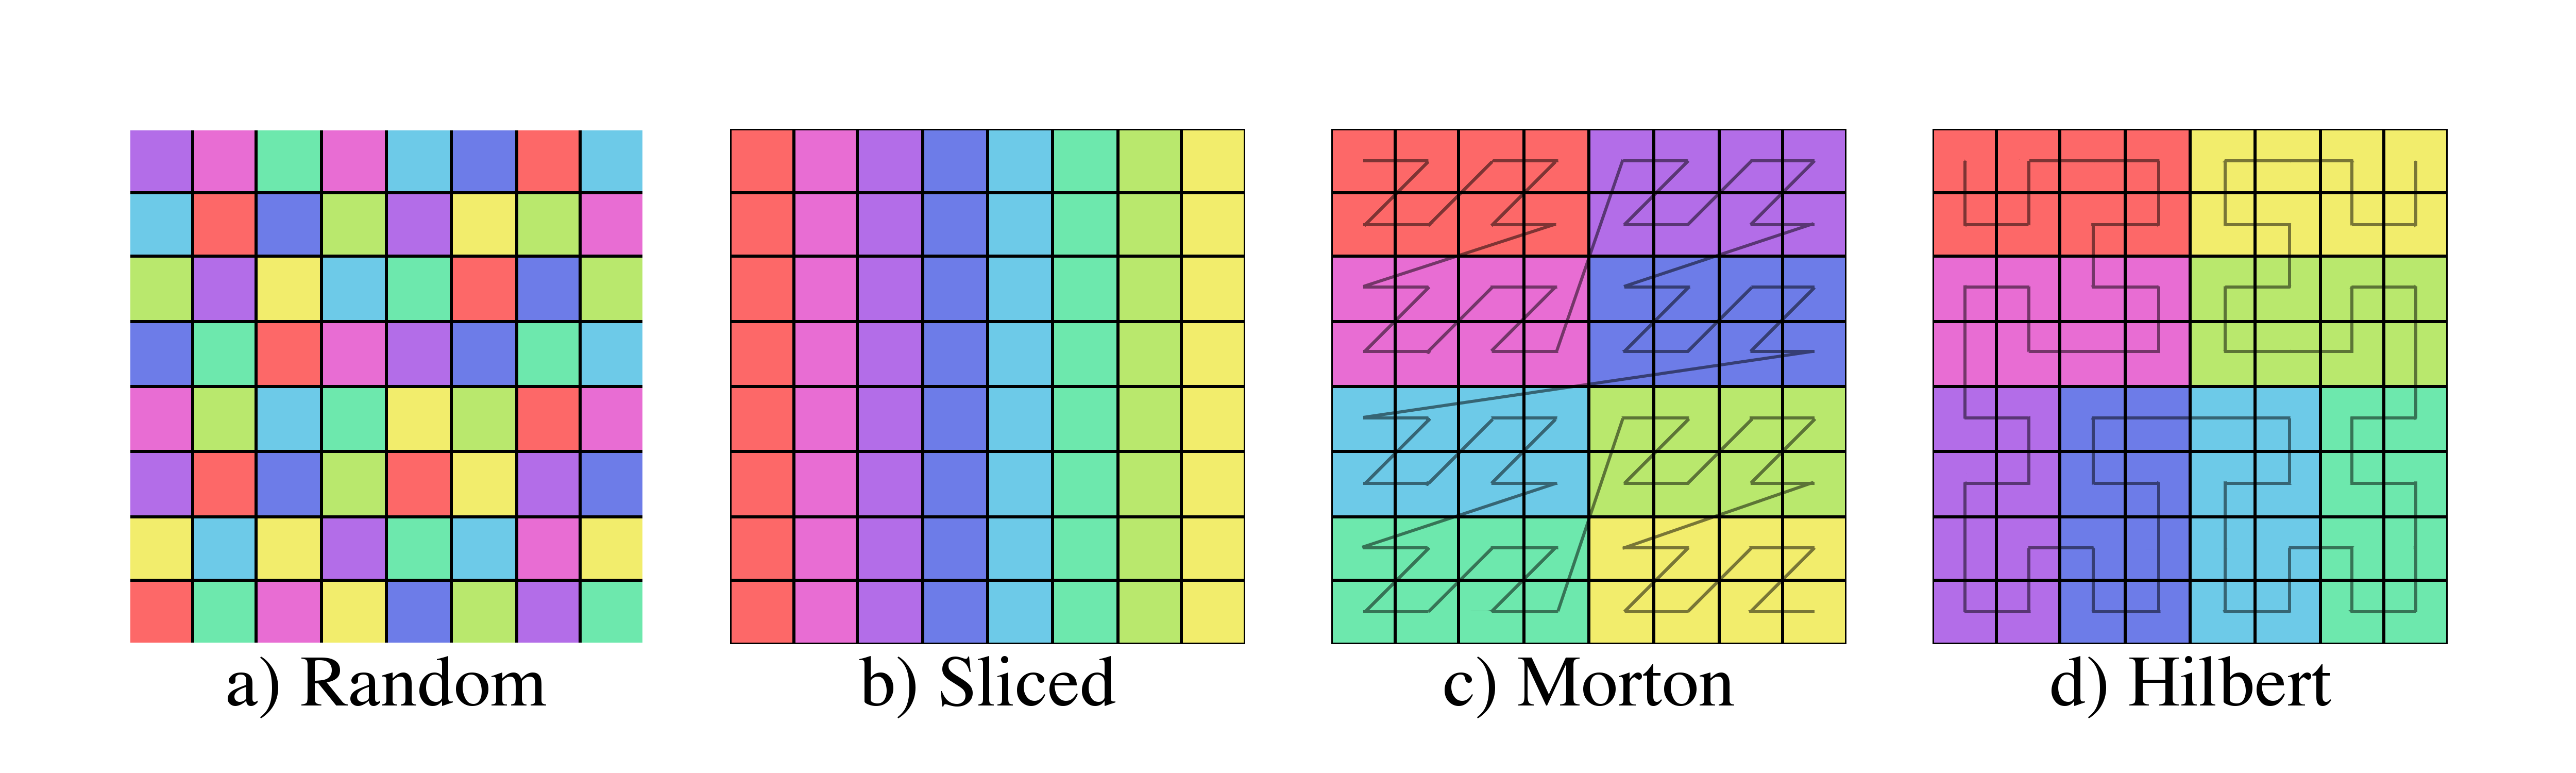
\includegraphics[width=\columnwidth,keepaspectratio]{../images/files.png}
\caption{Examples of four different schemes for partitioning a 2D domain between 8 files. Each color represents a different file.}
\label{fig:files}
\end{center}
\end{figure}
%

Panel (a) is an example where random parts of the domain are contained within each file. In such a case, many files will need to be loaded for contiguous selections within the domain. In panel (b), the domain was split between the files along the $x$ dimension. Fewer files will need to be loaded for queries along the $y$-dimension, but contiguous selection in $x$ will still require a greater number of files. Panels (c) and (d) are both examples of partitioning the domain between the files along a space filling curve (Morton and Hilbert curves respectively). These partitions have the greatest chance of limiting the number of files that must be loaded for a contiguous selection with slightly improved localization for the Hilbert curve. \todo{Examples of use cases \addref.}

Figure \ref{fig:selectors} shows examples of three selections within the above domain partitions. 
%
\begin{figure}[htbp]
\begin{center}
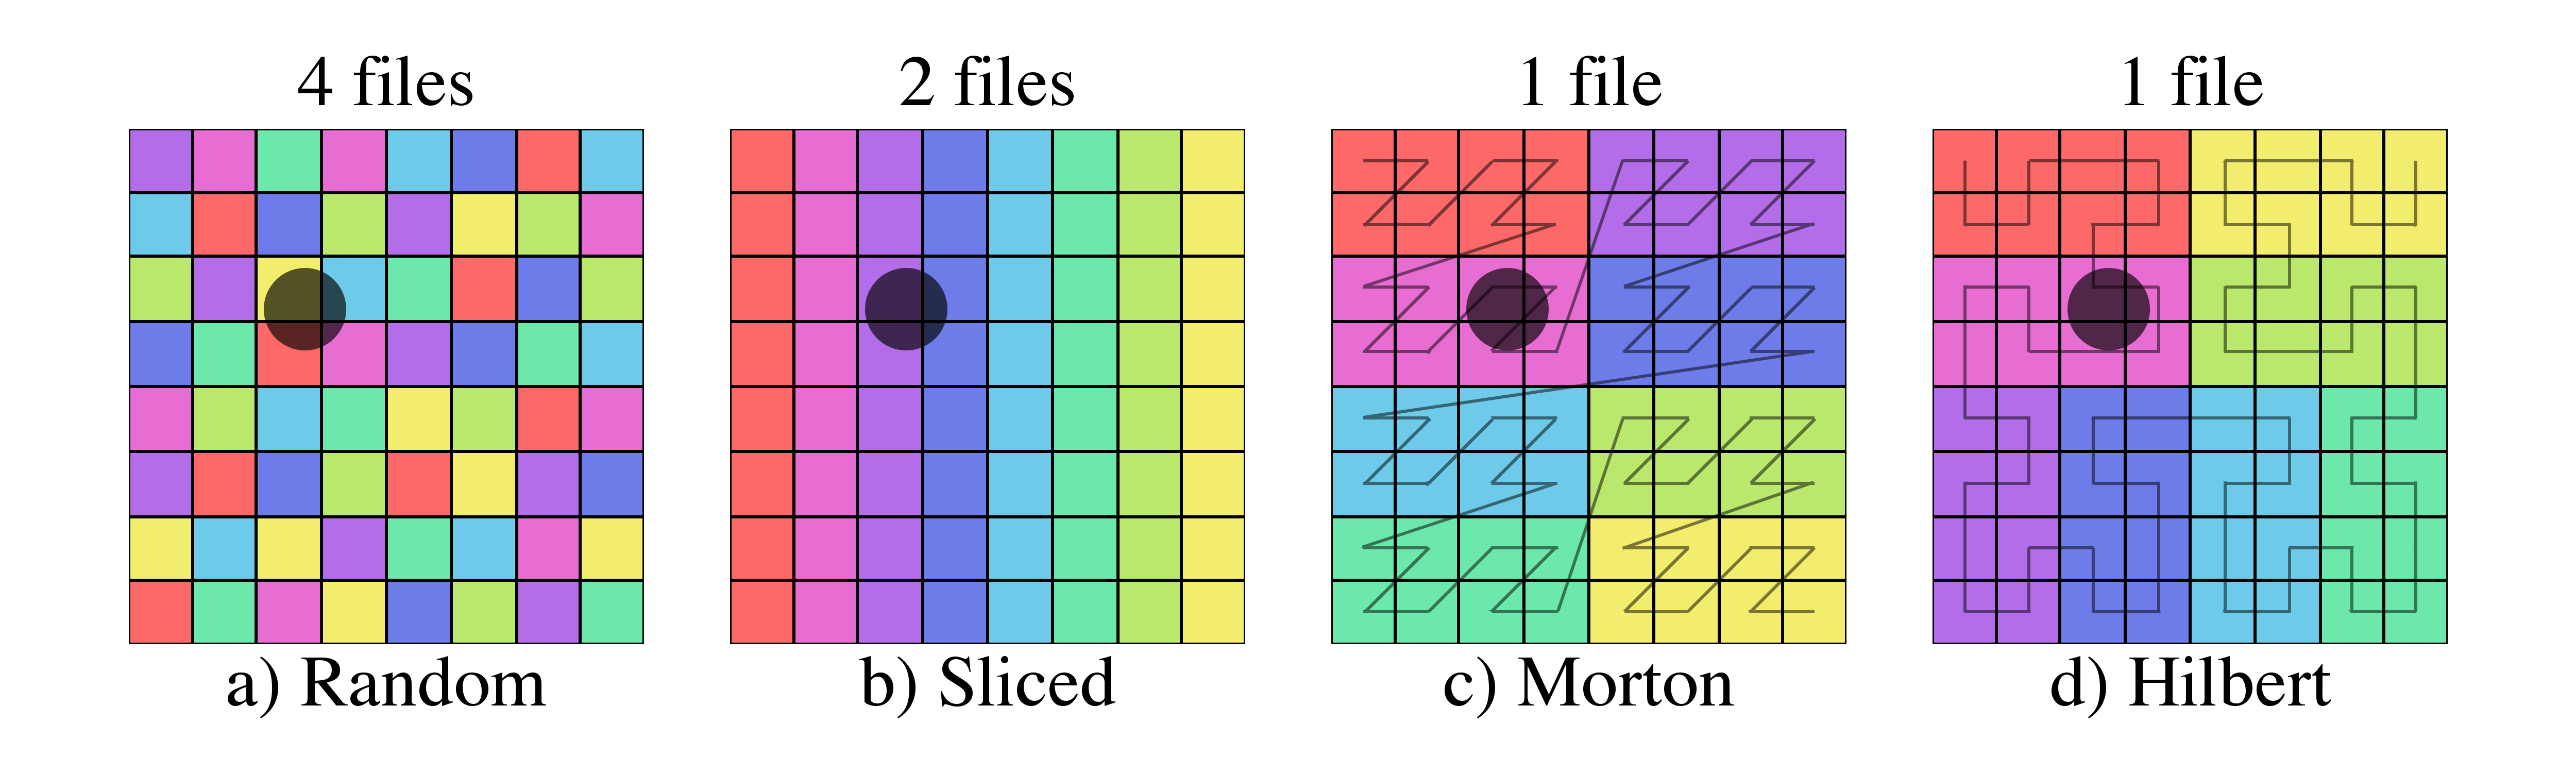
\includegraphics[width=\columnwidth,keepaspectratio]{../images/selector1.png}
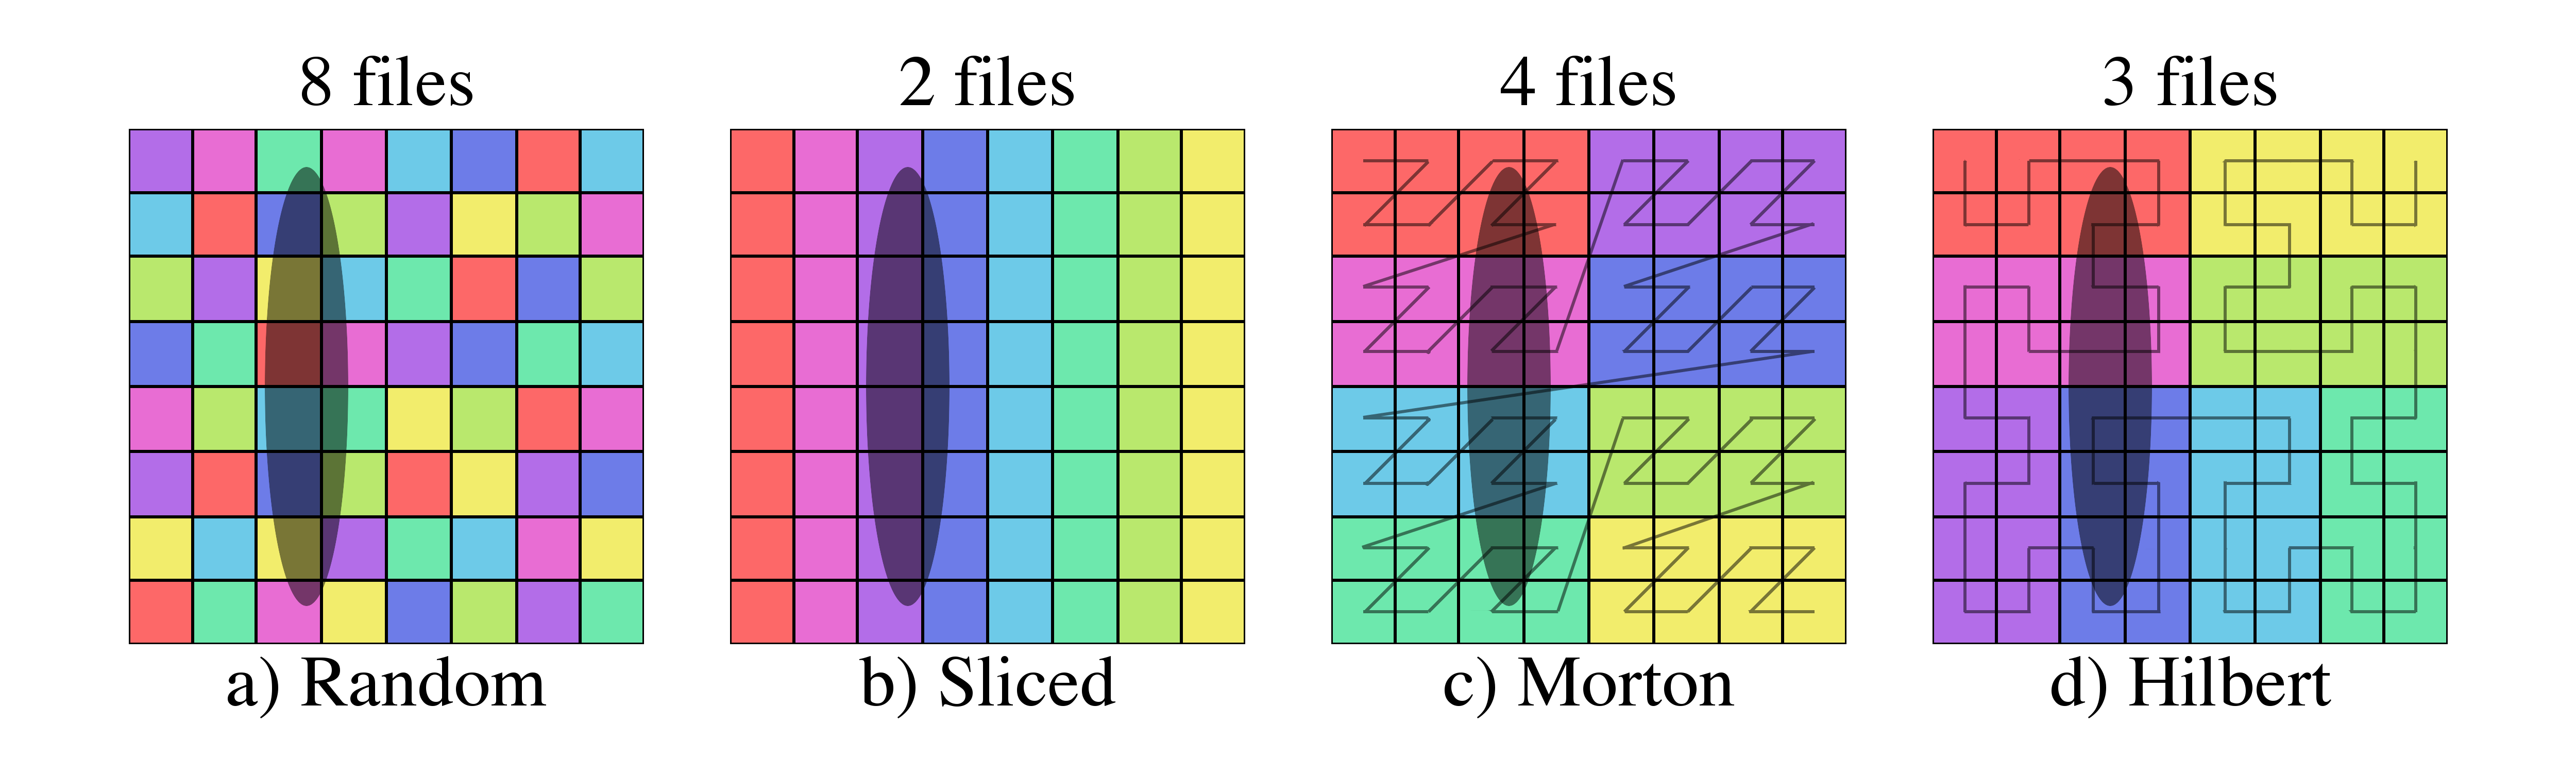
\includegraphics[width=\columnwidth,keepaspectratio]{../images/selector5.png}
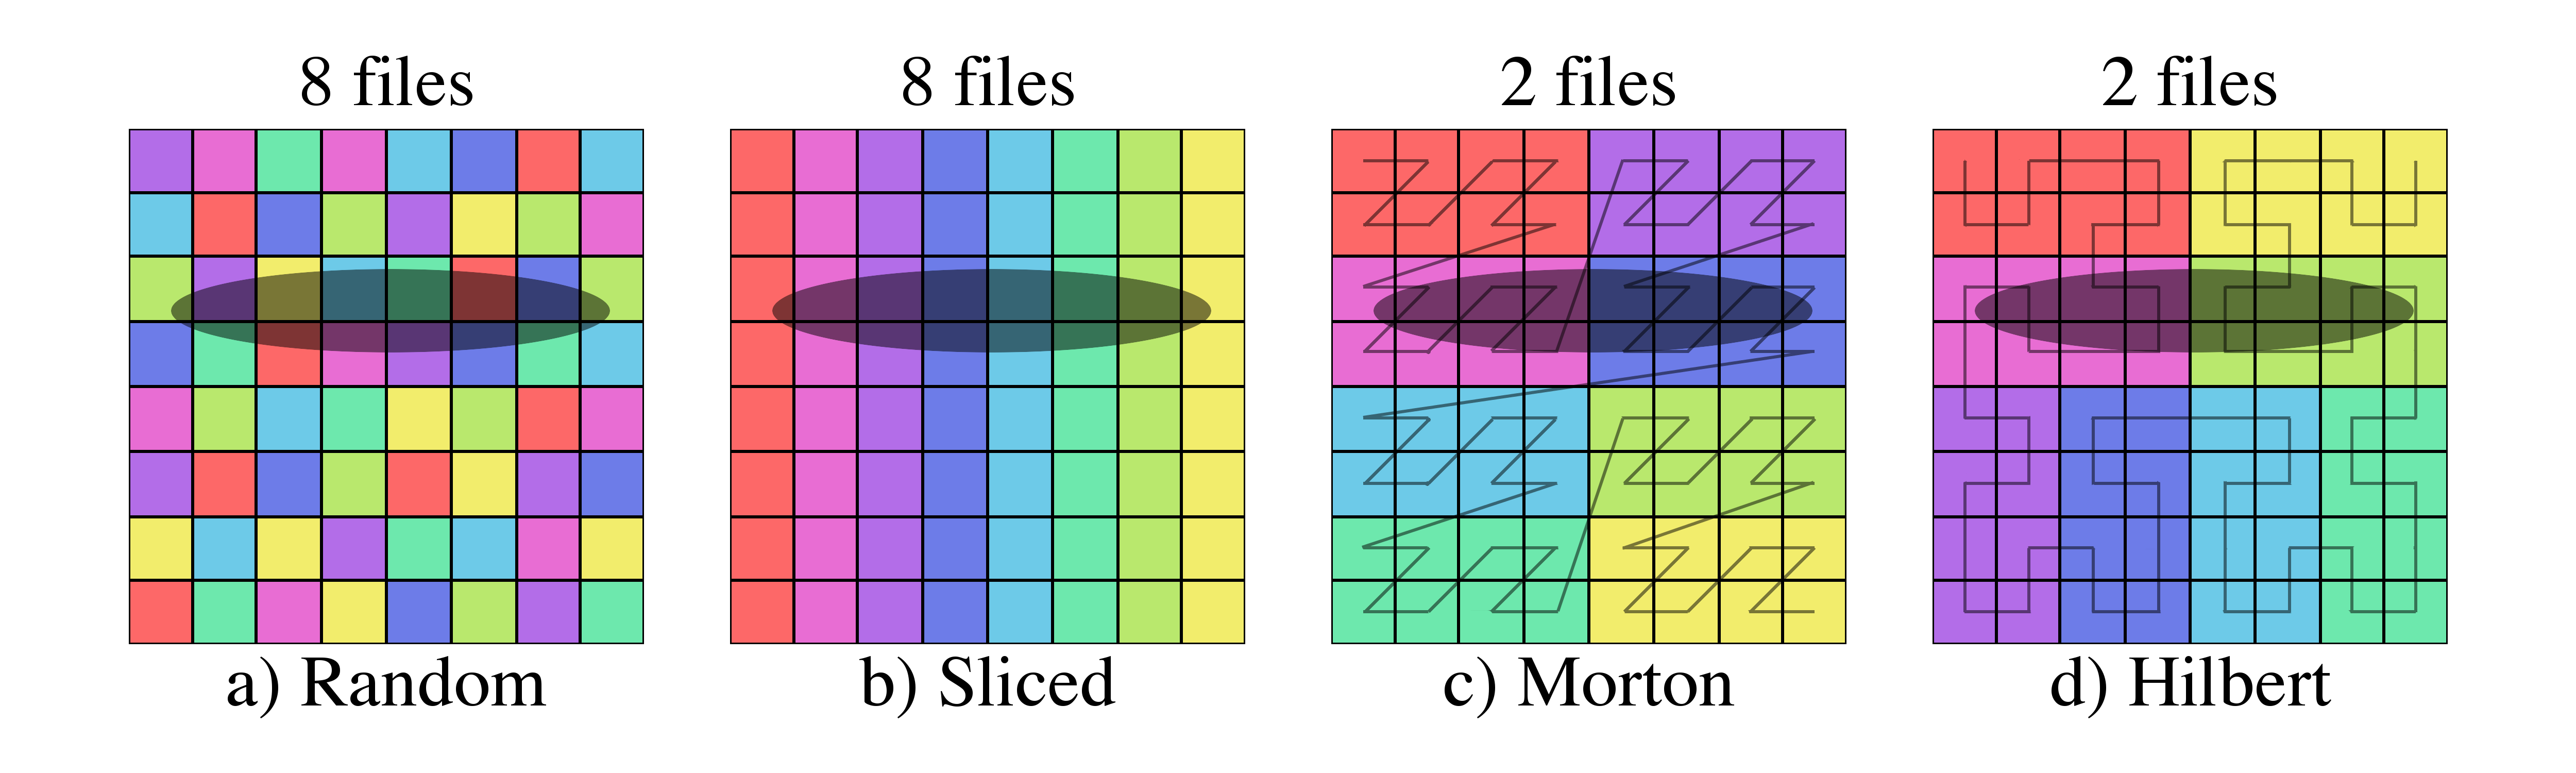
\includegraphics[width=\columnwidth,keepaspectratio]{../images/selector4.png}
\caption{Examples of file selection for four different domain partitions and three different selectors. The number of files above each images is the number of files that must be loaded in order to get all of the data within the selector.}
\label{fig:selectors}
\end{center}
\end{figure}
%
For the smallest selector (first row), the random domain decomposition (a) already requires half of the files to be loaded while more localized schemes require much fewer. Similarly, while the sliced domain partition (b), requires the fewest files to be loaded when the selector is oriented in the same direction as the slicing (second row), it requires all of the files when the selector is perpendicular to the slicing (third row). While some datasets may have information on the domain range covered by each file, the partitioning scheme used at output is often decided at runtime, can be system dependent, and may be imperfect. 

Files are often partitioned for parallel I/O such that each processor outputs data on the portion of the domain it is responsible for. To limit the cost of communication between processors, the domain will be split across processors such that neighboring processors are responsible for neighboring parts of the domain. This means that, although the overall partitioning scheme may be known for a given dataset, the exact order of the files will be dependent on the configuration of the processors at runtime. \addref

The partitioning can also be imperfect if the partition is not perfectly maintained. For instance, in astrophysical N-body simulations, it is possible for particles to travel from one processor's domain to another. In this case, the partition will only be perfect directly following an update to the domain decomposition. \addref

In cases where the exact file organization is not known or imperfect, it is advantageous to map the files post-process in order to speed up selections for analysis. 

%---------------------------------------------------------------------------------
% MORTON INDICES
\subsection{Morton Indices}
Morton order indices map multidimensional data onto a one-dimensional space filling curve \citep{Morton1996}. This is done by breaking up the domain into cells where each cell's position within the $N$-dimensional domain can be described by $N$ integers. The Morton index of the cell is then created by interleaving the bits of the $N$ integers to create a single integer that fully describes the cell's position (see Figure \ref{fig:zorder}). 
%
\begin{figure}[htbp]
\begin{center}
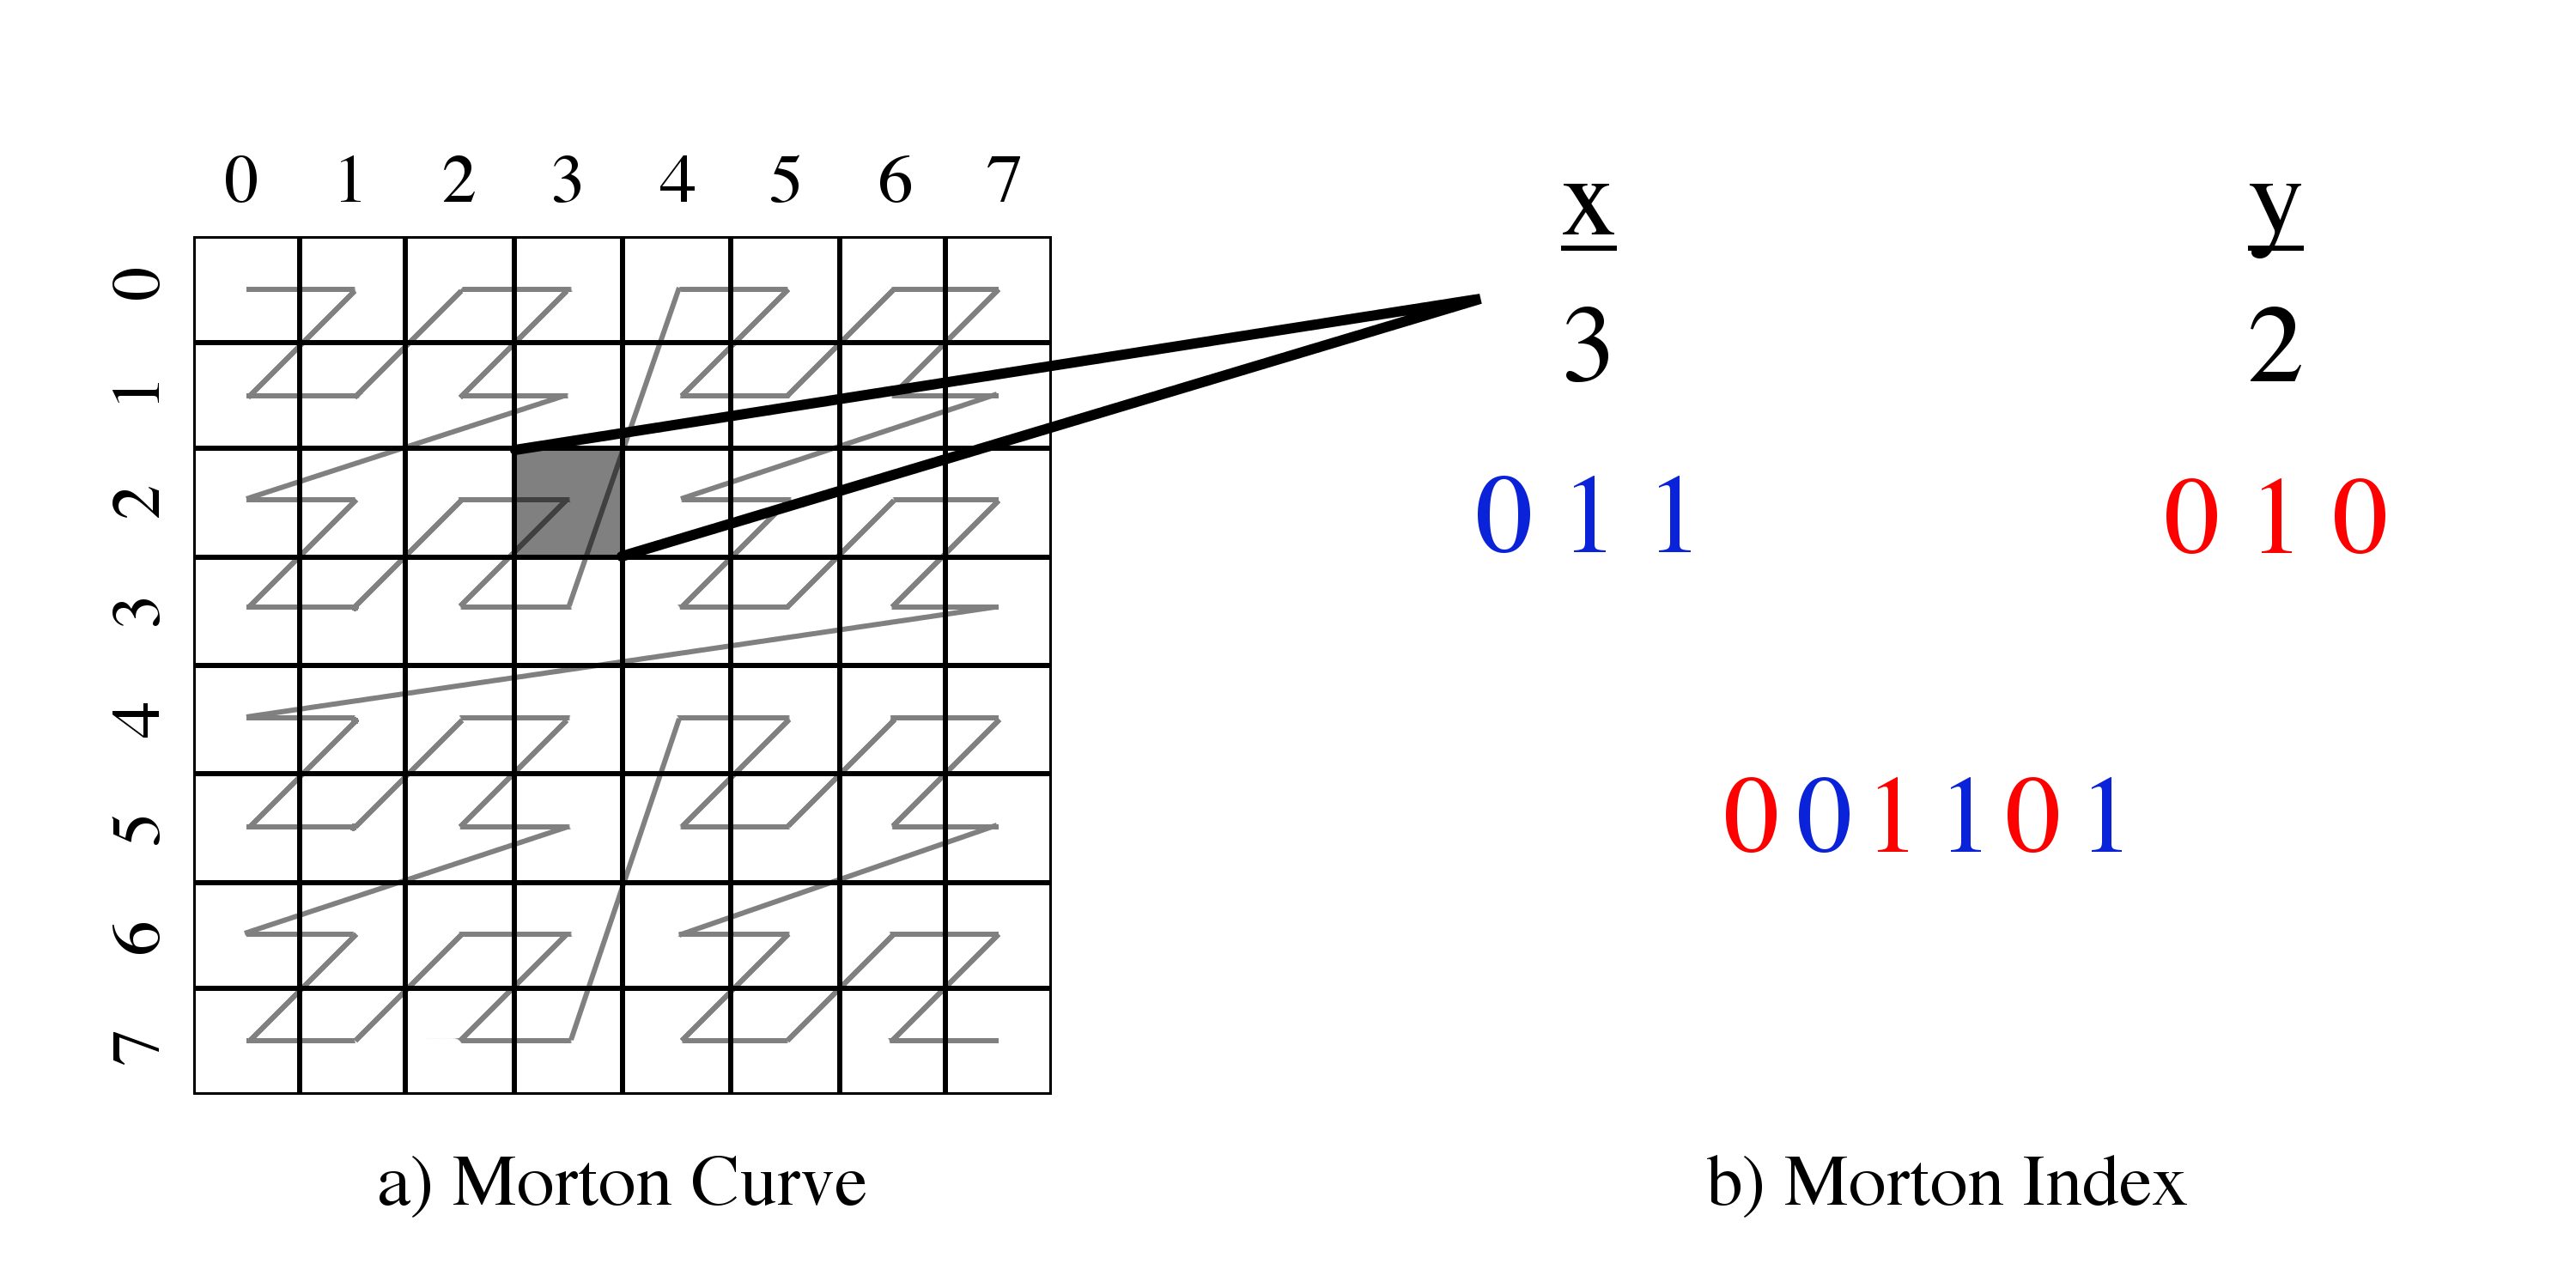
\includegraphics[width=0.75\columnwidth,keepaspectratio]{../images/zorder.png}
\caption{Example of 3rd order Morton curve. The bits of the $x$ and $y$ indices are interleaved to generate a single integer fully descriptive of it's location within the two-dimensional domain to within $1/2^{3}$th in each dimension.}
\label{fig:zorder}
\end{center}
\end{figure}
%

The precision of a single Morton index is only limited by the size of the integer used to store it. For instance, 64-bit Morton indices in 3 dimensions can be localized to $1/2^{21}$th of the domain in each dimension ($3\times21$\,bits = 63\,bits). If the domain is binarily divided into subcells to some order $k$ in each dimension (i.e. $2^{Nk}$ cells), coarser Morton indices can be obtained by simply masking lower bits. Morton indices can then be used to track what parts of the domain contain data and which files contain that data.

\todo{Examples of uses of Morton indices in the literature \addref.}

%---------------------------------------------------------------------------------
% BITMAPS & EWAH
\subsection{Bitmaps \& EWAH Compression}
For each file within a dataset, the Morton indices touched by the data can then be stored in a bitmap index for future searches where the value of bit $j$ indicates whether or not Morton index $j$ is touched by the file in question. For Morton indexing of order $k$, this would result in a bitmap of length $2^{Nk}$ bits per file. This can become costly in terms of memory and the time required to perform bitmap operations. However, Enhanced Word-Aligned Hybrid (EWAH) compression can be used to limit these costs, particularly when the domain is densely or sparsely populated in localized regions \citep{Wu2001,Lemire2010,Kaser2016}. 

An EWAH compressed bitmap will be smaller when there are long runs of identical values, with the smallest case being one in which either all or none of the bits are set. An uncompressed bitmap would require the same, maximum, amount of memory in both of these cases. The locality of Morton indices also takes advantage of the EWAH compression. If there are regions of the domain that are densely/sparsely populated, there Z-order space filling curve ensures that the bits denoting those regions will be adjacent, increasing the likelihood that there will be runs of identical (set/unset) bits.

%---------------------------------------------------------------------------------
% COLLISIONS
\subsection{Collisions}
It is possible that two files will contain data within the same Morton cell. This would mean that any time the data within that cell is accessed, both files would need to be loaded. Figure \ref{fig:collision} provides an example of collisions between two files. In panel (a) of Figure \ref{fig:collision}, purple cells are those that contain data from both files, a collision, for a 3rd order Morton index. Any selector that contained one of those cells would need to load all of the data from both files, even if it only selected part of the cell.
%
\begin{figure}[htbp]
\begin{center}
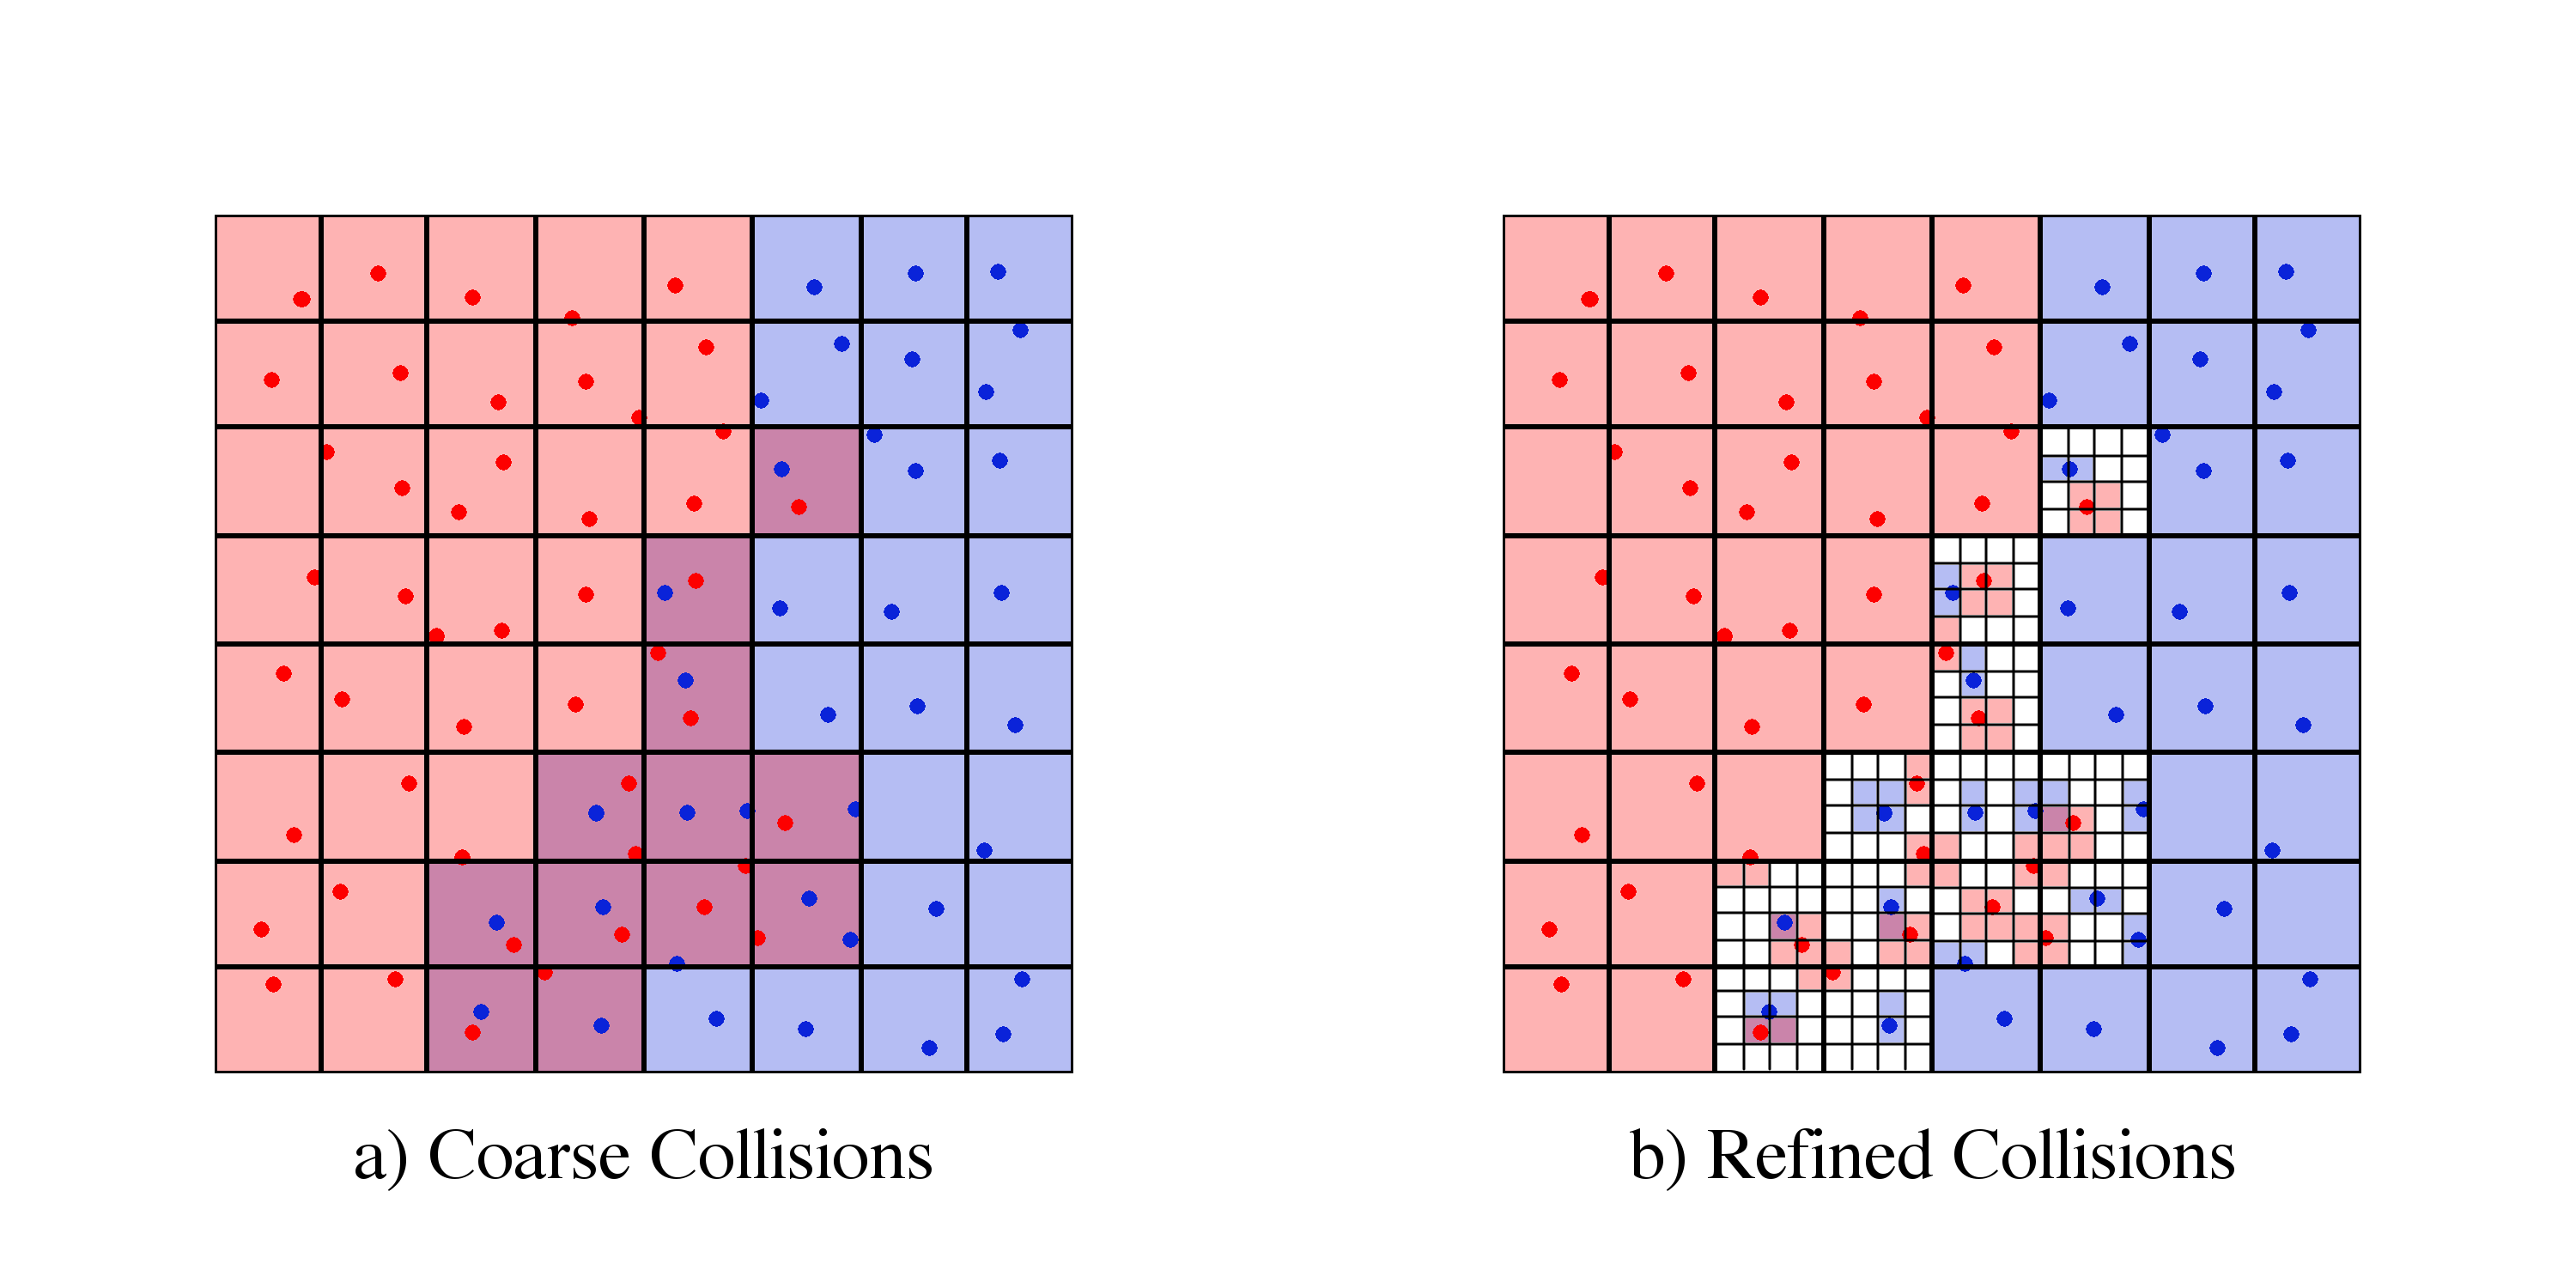
\includegraphics[width=\columnwidth,keepaspectratio]{../images/collisions.png}
\caption{Examples of a collision between two files. The red points and blue points are contained by two different files. The larger grid in both panels denotes the boundaries of 3rd order Morton cells.  The cells containing points from either file are shaded accordingly such that cells containing points from both files are purple. The smaller grids within these cells on the right are the boundaries of 2nd order Morton cells refining the collisions.}
\label{fig:collision}
\end{center}
\end{figure}
%

Collisions can be eliminated by either increasing the order of the index or nesting a second index within cells that contain collisions. This is demonstrated in panel (b) of Figure \ref{fig:collision}. In those cells which contained collisions, a 2nd order Morton index was added. Those cells with collisions at the level of the refined index (purple cells in panel (b)) cover a much smaller portion of the domain than the cells with collisions at the level of the coarse index (purple cells in panel (a)). This means that any given selection is less likely to contain a collision and it will be less likely for a selector to require both files to be loaded unless it actually touches data from both files.

Increasing the order of the coarse index has the same effect as nesting a second refined index within cells with collisions, but can also increases the size of the resulting map and the time it takes to identify files touched by a selection. However, if the order of the coarse index is too small or the order of the refined index too large, this too can increase the cost of a selection in terms of memory and time. \S\ref{SS:test_order} discusses this tradeoff and how to choose index orders.

Collisions are more common for file partitioning schemes that are not localized. Figure \ref{fig:collision_files} shows an example of collisions for the different partitioning schemes discussed in \S\ref{SS:decomp}.
%
\begin{figure}[htbp]
\begin{center}
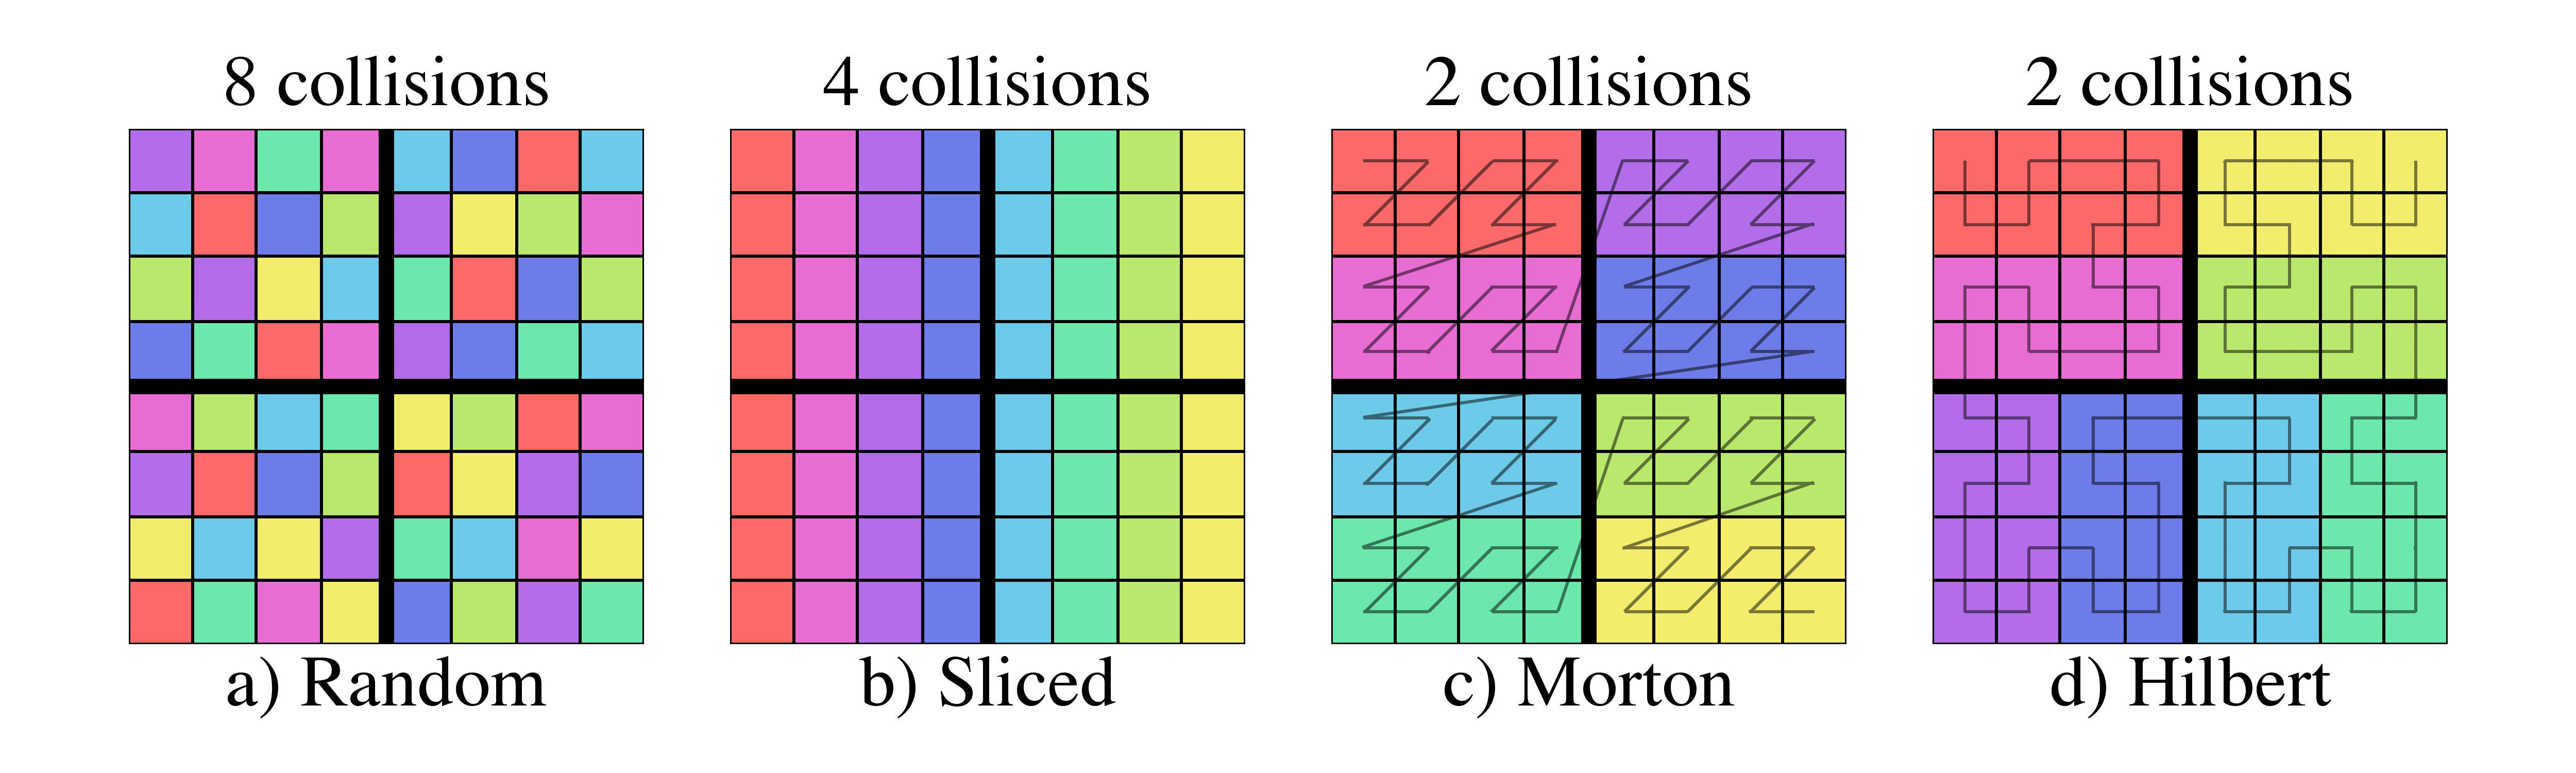
\includegraphics[width=\columnwidth,keepaspectratio]{../images/index.png}
\caption{Examples of collisions for four different domain partitioning schemes. The heavy black lines denote 1st order Morton cells. The presence of more that one file (color) within a Morton cell indicates a collision.}
\label{fig:collision_files}
\end{center}
\end{figure}
%
For the random domain partition in panel (a), every cell within a 1st order Morton index will contain data from all 8 files. This means that any selection using a 1st order bitmap index will require every file to be loaded. For the more localized partitions in panels (c) and (d), only two files touch each Morton cell.

%If collisions cannot be avoided, they can often be eliminated by either increasing the order of the Morton index or nesting a second index within the first (as in panel (b) of Figure \ref{fig:collision}). For instance, in Figure \ref{fig:collision_files}, if the index order were increased to 2, there would no longer be collisions in panels (c) and (d). While there would be fewer collisions in panels (a) and (b) for an index order of 2, an index order of 3 would be required to eliminate collisions entirely. While increasing the index order results in fewer collisions and will prevent files from being loaded unnecessarily, increasing the index order also increases the size of the resulting map and the time it takes to identify files touched be a selection (see \S\ref{SS:test_order} for a discussion of this tradeoff).

%---------------------------------------------------------------------------------
% GHOST ZONES
\subsection{Ghost Zones}
It is often the case that, in selecting a region, additional padding around the region should be included in the selection. This is particularly useful for algorithms that need information about neighboring points in the domain \addref. For Morton indices, this is straightforward as the indices neighboring Morton cells can be found by incrementing the bits corresponding to each dimension. We have included the ability to pad selectors with some number of Morton cells referred to as `ghost zones'. Those files that touch ghost zones, but not the selector itself are referred to below as `ghost files'. 

Depending on how the domain is split between files, the inclusion of ghost zones may or may not increase the number of files that need to be loaded. Figure \ref{fig:ghosts} shows an example of a ghost zone around the first selector from Figure \ref{fig:selectors}. 
%
\begin{figure}[htbp]
\begin{center}
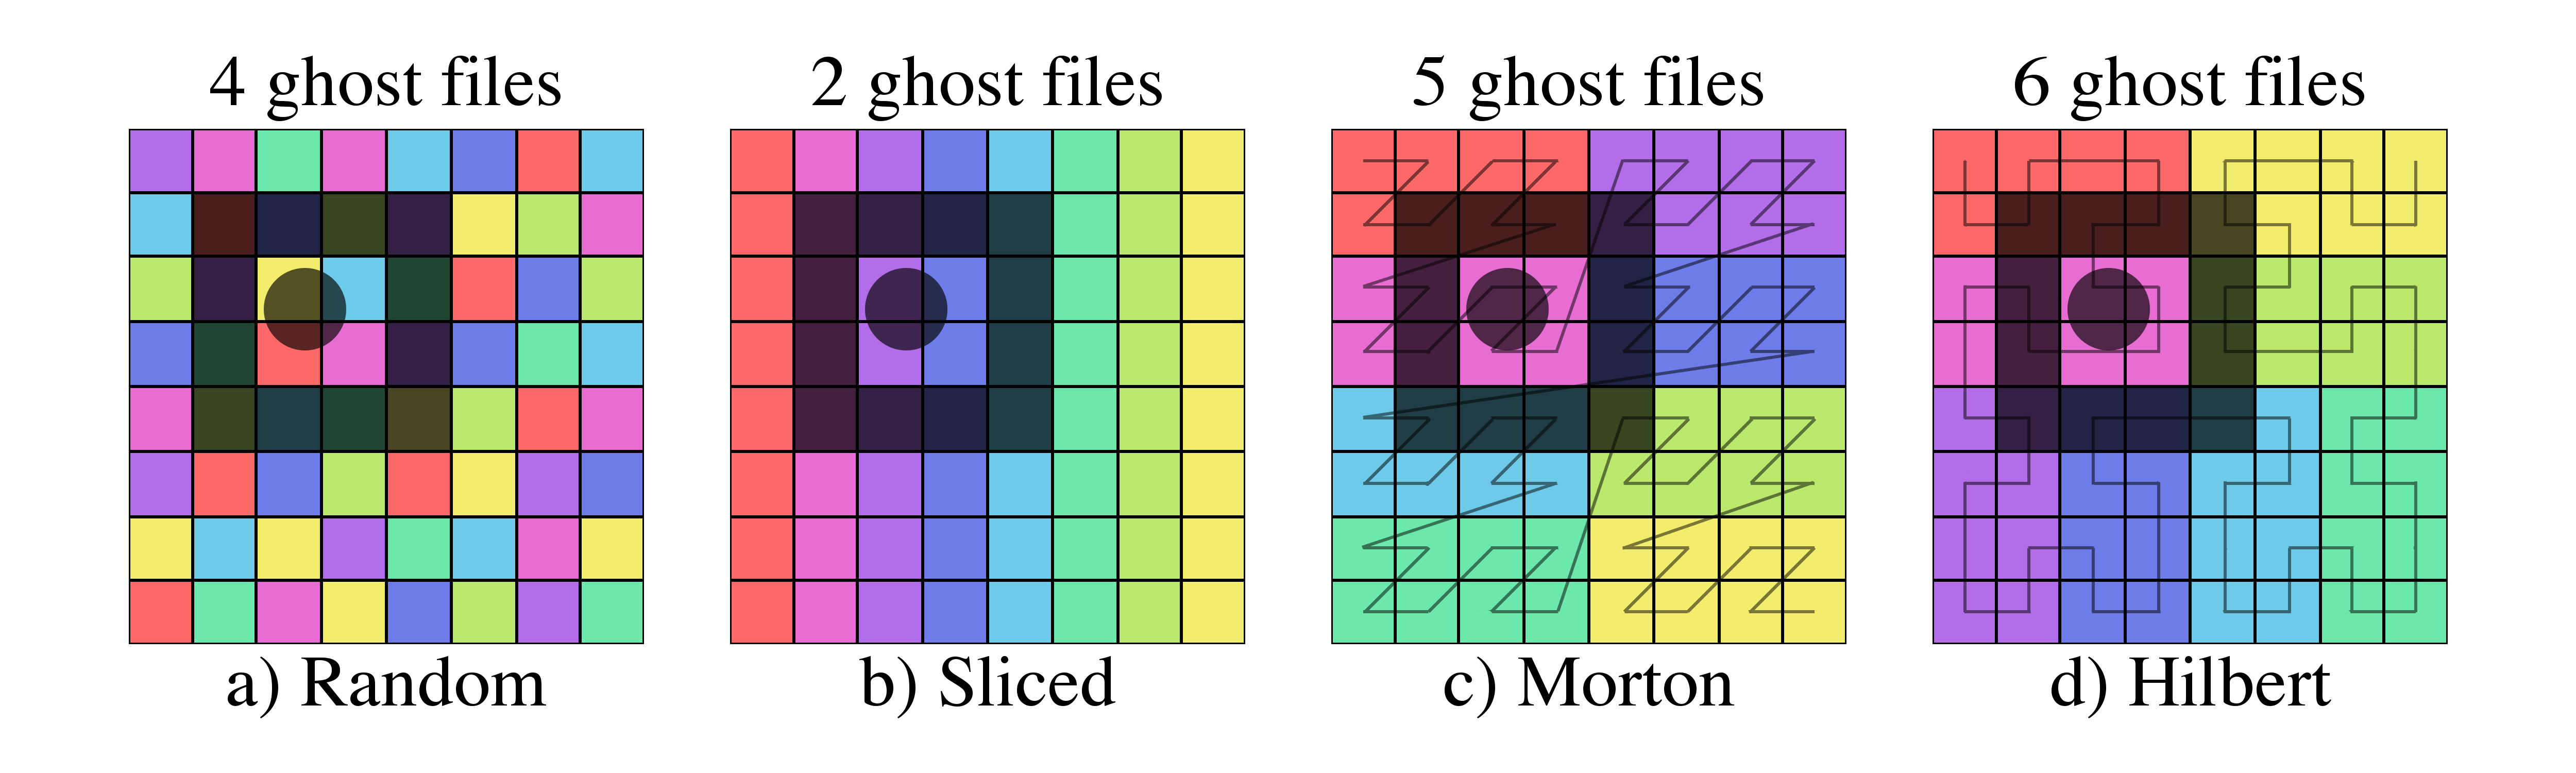
\includegraphics[width=\columnwidth,keepaspectratio]{../images/ghosts.png}
\caption{Examples of a selector ghost zone with a width of one Morton cell at an index order of 3 for  four different domain partitioning schemes. The shaded circular region is the selector and the shaded box is the ghost zone. Different partitioning schemes will lead to different numbers of ghost files.}
\label{fig:ghosts}
\end{center}
\end{figure}
%
The ghost zone has a width of one Morton cell at an index order of 3 and contains the same part of the domain in each case. However, due to differences in how the domain was partitioned between the files in the four cases, the number of additional ghost files touched by the ghost zone in each case is different. This will also depend on the order of the index to which ghost zones are added. Ghost zones added at the order of the coarse index will be larger than those added at the order of the refined index and will have a higher probability of touching additional files. While including ghost zones is advantageous when neighbor info is needed, it also increases the computational cost of identifying files (see \S\ref{S:tests}). 

%---------------------------------------------------------------------------------
%---------------------------------------------------------------------------------
% METHODS
\section{Methods}\label{S:methods}
The basic procedure for constructing the bitmap index is as follows:
\begin{enumerate}
\item {\bf Compute coarse indices.} For each file in the data set, read in the data and compute the indices of Morton cells at a given coarse order that are touched by data contained by that file. Store the coarse Morton indices in an EWAH compressed bitmap.
\item {\bf Find collisions.} Locate indices of coarse cells that are touched by data in more than one file (collisions) using bitwise operations. Record the collision indices in an EWAH compressed bitmap.
\item {\bf Compute refined indices.} For each file in the data set, read in the data and compute the indices Morton cells at a given refined order within coarse cells with collisions that are touched by data within that file. Store the refined Morton indices in a map from coarse Morton index to an EWAH compressed bitmap of refined Morton indices within that cell.
\item {\bf Output bitmaps.} Save EWAH compressed bitmaps for the coarse and refined indices contained with in each file in addition to the EWAH compressed bitmap containing the coarse indices with collisions.
\end{enumerate}

For large datasets and/or high order bitmaps, this can be a time consuming process. However, it must only be done once. For future selections, the bitmap can be quickly loaded and used to identify files in less time than would be required to load and query each file within the dataset individually. Selection using a loaded bitmap goes as follows:
\begin{enumerate}
\item {\bf Construct selector bitmap.} In the same way each file was mapped, the indices of Morton cells touched by the selector can be stored in a bitmap. This is done by checking for intersection of the selector with Morton cells at the order of the coarse bitmaps. For contiguous selectors, this can be done at lower order (parent) cells first and continued recursively until the order of the coarse bitmap is reached. 
\begin{itemize}
\item If a cell is completely within the selector, all of its child cells at the coarse order are added to the bitmap. 
\item If a cell intersects the edge of the selector, child cells at increasing orders are checked until the order of the coarse bitmaps are reached. 
\end{itemize}
If there is a collision between files within a coarse cell, a second order bitmap is constructed for the selector in the same manner.
\item {\bf Find files intersecting the selector.} Bitwise operations with the coarse file bitmaps can be used to efficiently identify files that intersect the selector within coarse cells. If the coarse cells within the intersection with a file all have collisions with other files, bitwise operations with the refined file bitmaps are then used to determine if the file is actually selected.
\end{enumerate}

If ghost zones are desired, the neighbors of cells that intersect the edge of the selector are added to a separate bitmap. For cells without collisions, the neighbors are added at the coarse bitmap order. If there are collisions, the neighbors are added at the refined bitmap order.

These procedures were implemented as part of the {\tt yt} python package \citep{Turk20d11a} in order to facilitate the analysis of large astrophysical N-body simulations. The open source EWAHBoolArray C++ package is used for implementing EWAH bitmaps \citep{Lemire2010,Kaser2016}.
\todo{more/separate code section...?}

%---------------------------------------------------------------------------------
%---------------------------------------------------------------------------------
% TESTS
\section{Tests}\label{S:tests}
The utility of using Morton index bitmaps for mapping files to decrease query times was tested on artificial datasets containing $1024^3$ points in three dimensions, distributed between 512 files. For each test a Morton index bitmap was constructed for the dataset and used to identify files touched by cube shaped three-dimensional selectors. The performance was then assessed in terms of the number of files touched and the time required to identify the files touched. If fewer files are touched, fewer files will need to be loaded during analysis of a selected region and the overall fraction of time spent on I/O will be lower. If less time is required to identify the files touched by a given selector, more selections can be made using the same computational resources. This was done for varying index orders (\S\ref{SS:test_order}), selector sizes (\S\ref{SS:test_size}), and partitions of the domain across the files (\S\ref{SS:test_decomp}).

% INDEX ORDER
% TOTAL REFINEMENT
\subsection{Index Order}\label{SS:test_order}
\subsubsection{Overall Refinement}\label{SSS:test_order1}
The order of the Morton indices used to map the files determines the time required to identify files and the number of collisions that will occur between files. Higher order indices will result in fewer collisions, but will take longer to query, as seen in Figure \ref{fig:test_order1}. Six selectors of varying sizes and positions within the domain where used to identify files based on Morton index bitmaps of varying order. The test dataset was split across the files using a Hilbert curve of order 6 with 10\% scatter between Hilbert cells to simulate an imperfect domain decomposition as can occur if particle positions are updated and output prior to communication.
%
\begin{figure}[htbp]
\begin{center}
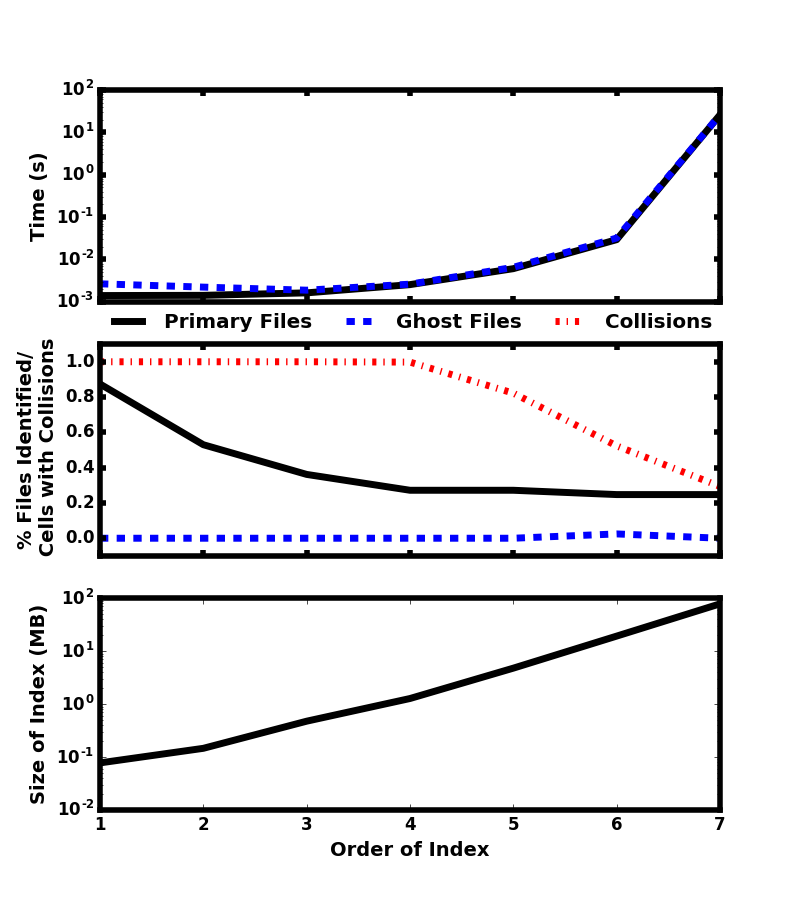
\includegraphics[width=\columnwidth,keepaspectratio]{../images/vary_order1_np1024_nf512_or0.png}
\caption{Dependence of query time (top) and fraction of files selected/cells with collisions (bottom) on total refinement of Morton indices. The solid black lines correspond to the query times and files identified by just the selectors. The dashed black lines correspond to the query times and additional files selected when a ghost zone with the width of one Morton cell is added around the selectors. The solid blue line in the bottom panel shows the fraction of cells with collisions between files.}
\label{fig:test_order1}
\end{center}
\end{figure}
%

Below an order of 4, there are collisions between multiple files for every index, resulting in a larger number of files being identified. However, as the order increases, the number of collisions drops and the file count plateaus at $\sim25$\%. For indices of order 7, selection requires $>100\times$ the time that the same selection took for an order of 6, but there is no change in the number of files indicated. For this dataset, an order of 6 is sufficient to identify the minimal set of files touched by the selectors. This is the order of the domain decomposition for the file partitioning.


% SECONDARY REFINEMENT
\subsubsection{Collision Refinement}\label{SSS:test_order2}
Increasing the refinement of the primary index does so for the entire domain and can become costly in terms of the memory required to store the bitmap and the time required to perform operations. However, it is also possible to increase refinement by nesting a second Morton index within those cells of the primary index that contain collisions. The resulting increase in memory and operations cost for adding the second index is then proportional to the number of collisions within the primary bitmap. This means that using a second index is only advantageous over increasing the order of the first index in some cases. Figure \ref{fig:test_order2} shows the results for adding a secondary index of varying order with the overall refinement order of the bitmap (primary index order + secondary index order) held constant at 6. The test dataset and selectors applied were the same as in \S\ref{SSS:test_order1}.
%
\begin{figure}[htbp]
\begin{center}
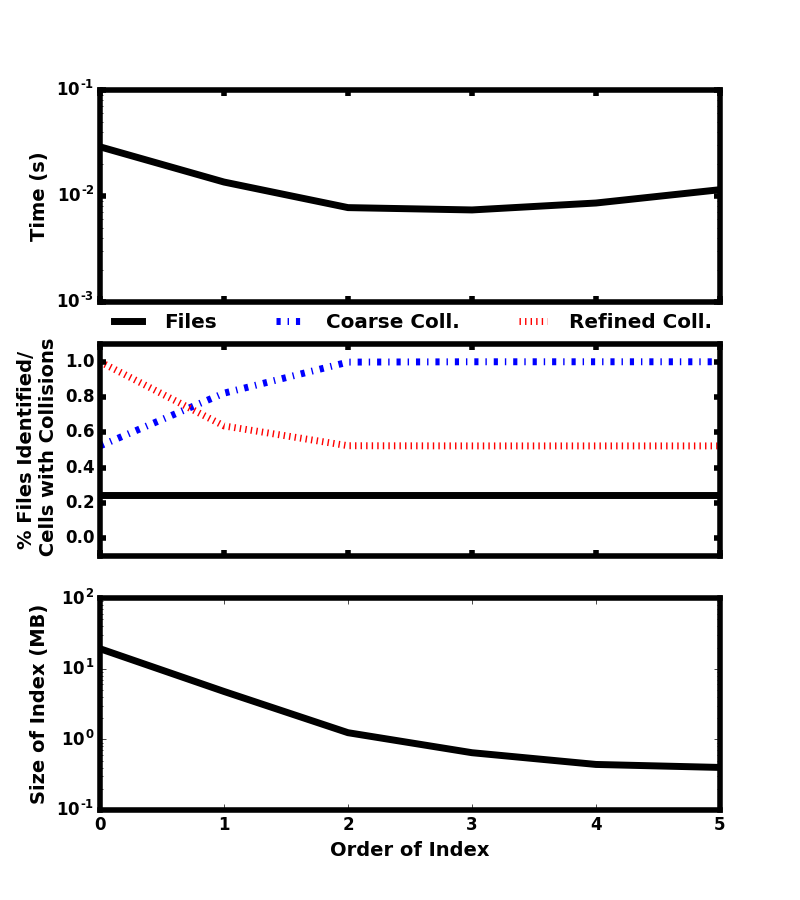
\includegraphics[width=\columnwidth,keepaspectratio]{../images/vary_order2_np1024_nf512.png}
\caption{Dependence of query time (top) and fraction of files selected/cells with collisions (bottom) on primary vs. secondary refinement. The solid black lines correspond to the query times and files identified. The dashed blue line in the bottom panel is the fraction of cells at the first index level that have collisions. The dotted blue line is the fraction of cells at the second index level that have collisions.}
\label{fig:test_order2}
\end{center}
\end{figure}
%

When the order of the second refined index is low, the first index is larger resulting in fewer cells with collisions at the first index and more at the second. The reverse is true when the order of second index is higher. As the overall order is held constant, the same number of files are identified regardless of the orders of the first and second indices. The time required to identify the files is minimized when cells within the first index become saturated with collisions. For higher order secondary indices, operations on the secondary bitmaps begin to be costly in terms of time for operations and memory consumption, but are still less expensive than in the case where only a single index is used. The optimal value for the orders of the first and second indexes will depend upon the dataset in question. The test dataset used here is uniformly distributed throughout the domain and does not need a high level of refinement at collisions. However, if a data set were less uniform with concentrations of points, the optimal order of the second index for performance may be higher.

% SELECTOR SIZE
\subsection{Selector Size}\label{SS:test_size}
%
The time required to identify files will also depend upon how large the selector is. Larger selectors will intersect more indices and more files, resulting in more bitmap operations. Figure \ref{fig:test_size} shows the result from varying the selector size. The same test data set from \S\ref{SS:test_order} was used. A bitmap with a primary Morton indices of order 4 and secondary Morton indices of order 2 were used in all cases. Each cube selector was placed at the center of the domain and scaled to some fraction of the total domain.
%
\begin{figure}[htbp]
\begin{center}
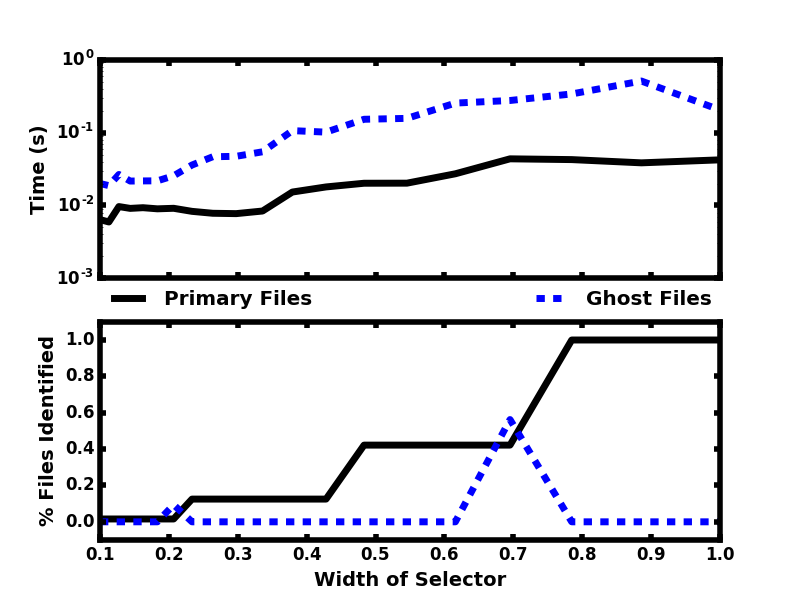
\includegraphics[width=\columnwidth,keepaspectratio]{../images/vary_selector_np1024_nf512.png}
\caption{Dependence of query time (top) and number of files selected (bottom) on selector width in terms of the total domain size. The solid black lines correspond to the query times and files identified by the selectors alone. The dashed black lines correspond the query times and additional files identified when a ghost zone with a width of one cell is added to the selector.}
\label{fig:test_size}
\end{center}
\end{figure}
%

As the selector increases in size, it touches a greater number of files, resulting in longer query times. The number of files touched increases in steps due to the way the test dataset was partitioned between files. Using the Hilbert curve, the domain cover by any one file is localized and will have a rectangular shape. This results in an order structure that is similar along all dimensions. An increases in the number of files touched indicates that the selector has grown past a file boundary in all directions. It is just prior to these jumps that ghost files are present. If the selector edge is near a file boundary, ghost zones have the potential to overlap the domains contained by neighboring files. For such a highly ordered dataset, the ghost zones will only identify additional files for selectors at the edges of file boundaries. However, queries including ghost zones require slightly more time even when this is not the case.


% DOMAIN DECOMP
\subsection{Domain Partitioning}\label{SS:test_decomp}
%
As discussed in \S\ref{SS:decomp}, the bitmap index is more effective in cases where the domain is partitioned between files in a localized way. If files contain non-contiguous parts of the domain, contiguous selections will require more files to be loaded. Figure \ref{fig:test_decomp} shows results for four different partitioning schemes. All four data sets cover the same three-dimensional domain with $1024^3$ points split across 512 files. The Hilbert dataset is the same one used in previous tests (see \S\ref{SS:test_order} for a description). The Morton dataset is constructed in a similar way to the Hilbert dataset with file partitions occurring along a 6th order Morton curve with 10\% scatter of points between Morton cells. The sliced dataset is partitioned in slices along one dimension with 10\% scatter of points between adjacent slices. Files in the random dataset contain a random sample of points, uniformly distributed across the domain.
%
\begin{figure}[hbpt]
\begin{center}
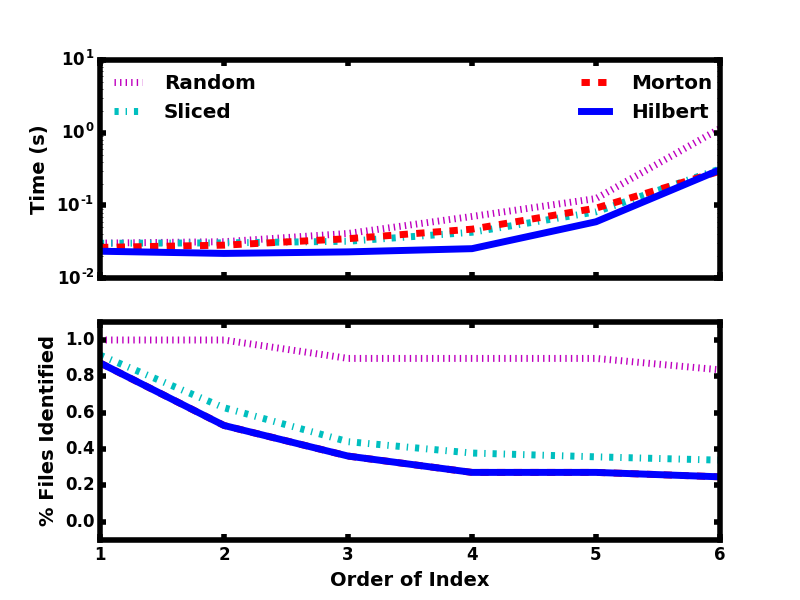
\includegraphics[width=\columnwidth,keepaspectratio]{../images/vary_decomp_np1024_nf512_or0.png}
\caption{Dependence of query time (top) and the number of files selected (bottom) on index order for different domain partitioning between files. The dotted magenta line is a randomly partitioned dataset, the cyan dashed-dotted line is a dataset partitioned by equal slices alone one dimension, the dashed red line is a dataset partitioned along an 6th order Morton curve, an the solid blue line is a dataset partitioned along a 6th order Hilbert curve.}
\label{fig:test_decomp}
\end{center}
\end{figure}

Many more files are identified for the random dataset than those datasets with localized partitioning of the domain. Above an order of 3, no additional files could be excluded for the random dataset. This was not true for the localized partitioning schemes. At the highest order, only $\sim20-30$\% of the files within these datasets would need to be loaded in order to get all of the data within the selected regions, while $>80$\% of the files in the random dataset would be required. The smallest fraction of files were identified for the Hilbert and Morton datasets, with a slightly greater fraction being identified for the sliced dataset. The sliced dataset performed particularly well in this case because the selectors used were cubes and did not preferentially select along any one dimension.

%---------------------------------------------------------------------------------
% SUMMARY & DISCUSSION
\section{Summary \& Discussion}\label{S:discuss}
Mapping files using Morton bitmap indexes speeds up analysis of large datasets split across multiple files by reducing the number of files that need to be loaded in order to perform operations on a subset of the full domain. The time required for making selections using the bitmap index is minimal for even large datasets and can be optimizing by partitioning the domain between files in a localized way and using an index or indexes of appropriate order for the dataset. 

Bitmap indexing is particularly useful in astronomy and astrophysics. Output from N-body simulations is often split between multiple files to take advantage of parallel I/O and the domain decomposition generally leads to localized partitioning between files \citep{Springel2001,Springel2005b,Hopkins2015}.\addref \todo{more}

\todo{applications outside astronomy}

Currently, this technique is most useful for datasets split across multiple files. However, it can also be applied to single files by dividing the file's contents into chunks. However, as in the multi-file case, the single file would need to be organized such that chunks were localized within the domain to take full advantage of the bitmaps.

%---------------------------------------------------------------------------------
% ACKNOWLEDGMENTS
\acknowledgments
\todo{write something}

%---------------------------------------------------------------------------------
% REFERENCES
\ifdraft
	\bibliography{Bitmap}
\else
	\begin{thebibliography}{10}

\bibitem{Croft2015}
R.~Croft, T.~{Di Matteo}, and N.~Khandai, ``{Petascale Cosmology: Simulations
  of Structure Formation},'' {\em Comput. Sci. Eng.}, vol.~17, pp.~40--46, mar
  2015.

\bibitem{Juric2015a}
M.~Juri{\'{c}}, J.~Kantor, K.-T. Lim, R.~H. Lupton, G.~Dubois-Felsmann,
  T.~Jenness, T.~S. Axelrod, J.~Aleksi{\'{c}}, R.~A. Allsman, Y.~AlSayyad,
  J.~Alt, R.~Armstrong, J.~Basney, A.~C. Becker, J.~Becla, S.~J. Bickerton,
  R.~Biswas, J.~Bosch, D.~Boutigny, M.~{Carrasco Kind}, D.~R. Ciardi, A.~J.
  Connolly, S.~F. Daniel, G.~E. Daues, F.~Economou, H.-F. Chiang, A.~Fausti,
  M.~Fisher-Levine, D.~M. Freemon, P.~Gee, P.~Gris, F.~Hernandez, J.~Hoblitt,
  {\v{Z}}.~Ivezi{\'{c}}, F.~Jammes, D.~Jevremovi{\'{c}}, R.~L. Jones, J.~{Bryce
  Kalmbach}, V.~P. Kasliwal, K.~S. Krughoff, D.~Lang, J.~Lurie, N.~B. Lust,
  F.~Mullally, L.~A. MacArthur, P.~Melchior, J.~Moeyens, D.~L. Nidever,
  R.~Owen, J.~K. Parejko, J.~M. Peterson, D.~Petravick, S.~R. Pietrowicz, P.~A.
  Price, D.~J. Reiss, R.~A. Shaw, J.~Sick, C.~T. Slater, M.~A. Strauss, I.~S.
  Sullivan, J.~D. Swinbank, S.~{Van Dyk}, V.~Vuj{\v{c}}i{\'{c}}, A.~Withers,
  P.~Yoachim, and {LSST Project}, ``{The LSST Data Management System},'' {\em
  eprint arXiv:1512.07914}, 2015.

\bibitem{Morton1996}
G.~M. Morton, ``{A computer oriented geodetic data base and a new technique in
  file sequencing},'' tech. rep., IBM Ltd., Ottawa, Ontario, 1996.

\bibitem{Hilbert1970}
D.~Hilbert, {\em {Gesammelte Abhandlungen: Band III: Analysis - Grundlagen der
  Mathematik Physik - Verschiedenes Lebensgeschichte}}, ch.~{\{}{\"{U}}{\}}ber
  die, pp.~1--2.
\newblock Berlin, Heidelberg: Springer Berlin Heidelberg, 1970.

\bibitem{Springel2005b}
V.~Springel, ``{The cosmological simulation code gadget-2},'' {\em Mon. Not. R.
  Astron. Soc.}, vol.~364, pp.~1105--1134, dec 2005.

\bibitem{Teyssier2001}
R.~Teyssier, ``{Cosmological Hydrodynamics with Adaptive Mesh Refinement: a new
  high resolution code called RAMSES},'' {\em Astron. Astrophys. v.385,
  p.337-364}, vol.~385, pp.~337--364, nov 2001.

\bibitem{Hjaltason2002}
G.~R. Hjaltason and H.~Samet, ``{Speeding up construction of PMR quadtree-based
  spatial indexes},'' {\em VLDB J. Int. J. Very Large Data Bases}, vol.~11,
  pp.~109--137, oct 2002.

\bibitem{Connor2010}
M.~Connor and P.~Kumar, ``{Fast construction of k-nearest neighbor graphs for
  point clouds.},'' {\em IEEE Trans. Vis. Comput. Graph.}, vol.~16,
  pp.~599--608, jan 2010.

\bibitem{Orenstein1984}
J.~A. Orenstein and T.~H. Merrett, ``{A class of data structures for
  associative searching},'' in {\em Proc. 3rd ACM SIGACT-SIGMOD Symp. Princ.
  database Syst. - Pod. '84}, (New York, New York, USA), p.~181, ACM Press, apr
  1984.

\bibitem{Wu1998}
M.-C. Wu and A.~Buchmann, ``{Encoded bitmap indexing for data warehouses},'' in
  {\em Proc. 14th Int. Conf. Data Eng.}, pp.~220--230, IEEE Comput. Soc, 1998.

\bibitem{Chan1998}
C.-Y. Chan and Y.~E. Ioannidis, ``{Bitmap index design and evaluation},'' {\em
  ACM SIGMOD Rec.}, vol.~27, pp.~355--366, jun 1998.

\bibitem{Chan1999}
C.-Y. Chan and Y.~E. Ioannidis, ``{An efficient bitmap encoding scheme for
  selection queries},'' {\em ACM SIGMOD Rec.}, vol.~28, pp.~215--226, jun 1999.

\bibitem{Malensek2014}
M.~Malensek, S.~Pallickara, and S.~Pallickara, ``{Evaluating Geospatial
  Geometry and Proximity Queries Using Distributed Hash Tables},'' {\em Comput.
  Sci. Eng.}, vol.~16, pp.~53--61, jul 2014.

\bibitem{Sinha2006}
R.~Sinha, S.~Mitra, and M.~Winslett, ``{Bitmap indexes for large scientific
  data sets: a case study},'' in {\em Proc. 20th IEEE Int. Parallel Distrib.
  Process. Symp.}, p.~10 pp., IEEE, 2006.

\bibitem{Sinha2007}
R.~R. Sinha and M.~Winslett, ``{Multi-resolution bitmap indexes for scientific
  data},'' {\em ACM Trans. Database Syst.}, vol.~32, pp.~16--es, aug 2007.

\bibitem{Stockinger2000}
K.~Stockinger, D.~Duellmann, W.~Hoschek, and E.~Schikuta, ``{Improving the
  Performance of High-Energy Physics Analysis through Bitmap Indices},'' in
  {\em Database Expert Syst. Appl. 11th Int. Conf. DEXA 2000 London, UK, Sept.
  4--8, 2000 Proc.} (M.~Ibrahim, J.~K{\"{u}}ng, and N.~Revell, eds.), vol.~1873
  of {\em Lecture Notes in Computer Science}, ch.~Improving, pp.~835--845,
  Berlin, Heidelberg: Springer Berlin Heidelberg, jun 2000.

\bibitem{Wu2003}
K.~Wu, W.~Koegler, J.~Chen, and A.~Shoshani, ``{Using bitmap index for
  interactive exploration of large datasets},'' in {\em 15th Int. Conf. Sci.
  Stat. Database Manag. 2003.}, pp.~65--74, IEEE Comput. Soc, 2003.

\bibitem{Yu1998}
P.~Yu, ``{Range-based bitmap indexing for high cardinality attributes with
  skew},'' in {\em Proceedings. Twenty-Second Annu. Int. Comput. Softw. Appl.
  Conf. (Compsac '98) (Cat. No.98CB 36241)}, pp.~61--66, IEEE Comput. Soc,
  1998.

\bibitem{Shoshani1999}
A.~Shoshani, L.~Bernardo, H.~Nordberg, D.~Rotem, and A.~Sim,
  ``{Multidimensional indexing and query coordination for tertiary storage
  management},'' in {\em Proceedings. Elev. Int. Conf. Sci. Stat. Database
  Manag.}, pp.~214--225, IEEE Comput. Soc, 1999.

\bibitem{Stockinger2004}
K.~Stockinger, K.~Wu, and A.~Shoshani, ``{Evaluation Strategies for Bitmap
  Indices with Binning},'' in {\em Database Expert Syst. Appl. 15th Int. Conf.
  DEXA 2004, Zaragoza, Spain, August 30-September 3, 2004. Proc.} (F.~Galindo,
  M.~Takizawa, and R.~Traunm{\"{u}}ller, eds.), (Berlin, Heidelberg),
  pp.~120--129, Springer Berlin Heidelberg, 2004.

\bibitem{Wu2001}
K.~Wu, E.~Otoo, and A.~Shoshani, ``{Compressed bitmap indices for efficient
  query processing},'' {\em Lawrence Berkeley Natl. Lab.}, sep 2001.

\bibitem{Lemire2010}
D.~Lemire, O.~Kaser, and K.~Aouiche, ``{Sorting improves word-aligned bitmap
  indexes},'' {\em Data Knowl. Eng.}, vol.~69, pp.~3--28, jan 2010.

\bibitem{Kaser2016}
O.~Kaser and D.~Lemire, ``{Compressed bitmap indexes: beyond unions and
  intersections},'' {\em Softw. Pract. Exp.}, vol.~46, pp.~167--198, feb 2016.

\bibitem{Monaghan1992}
J.~J. Monaghan, ``{Smoothed Particle Hydrodynamics},'' {\em Annu. Rev. Astron.
  Astrophys.}, vol.~30, pp.~543--574, sep 1992.

\bibitem{Springel2001}
V.~Springel, N.~Yoshida, and S.~D.~M. White, ``{GADGET: a code for
  collisionless and gasdynamical cosmological simulations},'' {\em New
  Astron.}, vol.~6, pp.~79--117, apr 2001.

\bibitem{Hopkins2015}
P.~F. Hopkins, ``{A new class of accurate, mesh-free hydrodynamic simulation
  methods},'' {\em Mon. Not. R. Astron. Soc.}, vol.~450, pp.~53--110, apr 2015.

\bibitem{Turk20d11a}
M.~J. Turk, B.~D. Smith, J.~S. Oishi, S.~Skory, S.~W. Skillman, T.~Abel, and
  M.~L. Norman, ``{yt: A MULTI-CODE ANALYSIS TOOLKIT FOR ASTROPHYSICAL
  SIMULATION DATA},'' {\em Astrophys. J. Suppl. Ser.}, vol.~192, p.~9, jan
  2011.

\bibitem{Behnel2011}
S.~Behnel, R.~Bradshaw, C.~Citro, L.~Dalcin, D.~S. Seljebotn, and K.~Smith,
  ``{Cython: The Best of Both Worlds},'' {\em Comput. Sci. Eng.}, vol.~13,
  pp.~31--39, mar 2011.

\end{thebibliography}

\fi

%---------------------------------------------------------------------------------
% FIGURES
\ifplacefig
\else
% put figures here if figures go after
\fi

%---------------------------------------------------------------------------------
% COMMENTS
\newpage
\todo{To do:
\begin{itemize}
\item Improve introduction \& conclusion
\item Find \& add tagged references.
\item Acknowledgements
\item Switch times for tests to be averages over 10 runs (with std. dev. error bars?)
\item Make diagram showing buffer added to test datasets?
\item Plot \% files identified vs. \% domain selected?
\item Ensure plot labels are all the same size when in document (set widths to colsize)
\end{itemize}
}

\end{document}
